% Template file for an a0 landscape poster.
% Written by Graeme, 2001-03 based on Norman's original microlensing
% poster.
%
% See discussion and documentation at
% <http://www.astro.gla.ac.uk/users/norman/docs/posters/> 
%
% $Id: poster-template-landscape.tex,v 1.2 2002/12/03 11:25:46 norman Exp $


% Default mode is landscape, which is what we want, however dvips and
% a0poster do not quite do the right thing, so we end up with text in
% landscape style (wide and short) down a portrait page (narrow and
% long). Printing this onto the a0 printer chops the right hand edge.
% However, 'psnup' can save the day, reorienting the text so that the
% poster prints lengthways down an a0 portrait bounding box.
%
% 'psnup -w85cm -h119cm -f poster_from_dvips.ps poster_in_landscape.ps'

\documentclass[a0]{a0poster}
% You might find the 'draft' option to a0 poster useful if you have
% lots of graphics, because they can take some time to process and
% display. (\documentclass[a0,draft]{a0poster})
\input defs
\pagestyle{empty}
\setcounter{secnumdepth}{0}
\renewcommand{\familydefault}{\sfdefault}
\newcommand{\QED}{~~\rule[-1pt]{8pt}{8pt}}\def\qed{\QED}

\renewcommand{\reals}{{\mbox{\bf R}}}

% The textpos package is necessary to position textblocks at arbitary 
% places on the page.
\usepackage[absolute]{textpos}

\usepackage{fleqn,psfrag,wrapfig,tikz,amsmath, framed, scrextend,subcaption}
\usepackage{mathtools,url}
\DeclarePairedDelimiterX{\norm}[1]{\lVert}{\rVert}{#1}

\usepackage[papersize={38in,28in}]{geometry}

% Graphics to include graphics. Times is nice on posters, but you
% might want to switch it off and go for CMR fonts.
\usepackage{graphics}

\renewenvironment{leftbar}[1][\hsize]
{% 
\def\FrameCommand 
{%

    {\color{black}\vrule width 0pt}%
    \hspace{0pt}%must no space.
    \fboxsep=\FrameSep\colorbox{white}%
}%
\MakeFramed{\hsize#1\advance\hsize-\width\FrameRestore}%
}
{\endMakeFramed}

% we are running pdflatex, so convert .eps files to .pdf
%\usepackage[pdftex]{graphicx}
%\usepackage{epstopdf}

% These colours are tried and tested for titles and headers. Don't
% over use color!
\usepackage{color}
\definecolor{Red}{rgb}{0.9,0.0,0.1}

\definecolor{bluegray}{rgb}{0.15,0.20,0.40}
\definecolor{bluegraylight}{rgb}{0.35,0.40,0.60}
\definecolor{gray}{rgb}{0.3,0.3,0.3}
\definecolor{lightgray}{rgb}{0.7,0.7,0.7}
\definecolor{darkblue}{rgb}{0.2,0.2,1.0}
\definecolor{darkgreen}{rgb}{0.0,0.5,0.3}

\renewcommand{\labelitemi}{\textcolor{bluegray}\textbullet}
\renewcommand{\labelitemii}{\textcolor{bluegray}{--}}

\setlength{\labelsep}{0.5em}


% see documentation for a0poster class for the size options here
\let\Textsize\normalsize
%\def\Head#1{\noindent\hbox to \hsize{\hfil{\LARGE\color{bluegray} #1}}\bigskip}
\def\Head#1{\noindent{\LARGE\color{bluegray} #1}\bigskip}
\def\LHead#1{\noindent{\LARGE\color{bluegray} #1}\bigskip}
\def\Subhead#1{\noindent{\large\color{bluegray} #1}\bigskip}
\def\Title#1{\noindent{\VeryHuge\color{Red} #1}}

\usepackage{multicol}
\setlength{\columnsep}{1cm}
\usepackage{vwcol} 
\usepackage{booktabs}

% Set up the grid
%
% Note that [40mm,40mm] is the margin round the edge of the page --
% it is _not_ the grid size. That is always defined as 
% PAGE_WIDTH/HGRID and PAGE_HEIGHT/VGRID. In this case we use
% 23 x 12. This gives us three columns of width 7 boxes, with a gap of
% width 1 in between them. 12 vertical boxes is a good number to work
% with.
%
% Note however that texblocks can be positioned fractionally as well,
% so really any convenient grid size can be used.
%
\TPGrid[40mm,40mm]{23}{12}      % 3 cols of width 7, plus 2 gaps width 1

\parindent=0pt
\parskip=0.2\baselineskip

\begin{document}

% Understanding textblocks is the key to being able to do a poster in
% LaTeX. In
%
%    \begin{textblock}{wid}(x,y)
%    ...
%    \end{textblock}
%
% the first argument gives the block width in units of the grid
% cells specified above in \TPGrid; the second gives the (x,y)
% position on the grid, with the y axis pointing down.

% You will have to do a lot of previewing to get everything in the 
% right place.

% This gives good title positioning for a portrait poster.
% Watch out for hyphenation in titles - LaTeX will do it
% but it looks awful.
\begin{textblock}{23}(0,0)
\Title{Player Behavior and Optimal Team Compositions in Online Games}
\end{textblock}

\begin{textblock}{23}(0,0.6)
{
\LARGE
Hao Yi Ong,
Sunil Deolalikar, and
Mark Peng
}

{
\Large
\color{bluegray}
\emph{CS 229: Machine Learning Class Project}
}
\end{textblock}


% Uni logo in the top right corner. A&A in the bottom left. Gives a
% good visual balance, but you may want to change this depending upon
% the graphics that are in your poster.
%\begin{textblock}{2}(0,10)
%Your logo here
%%\includegraphics{/usr/local/share/images/AandA.epsf}
%\end{textblock}

% \begin{textblock}{3}(21.0,0)
% % Another logo here
% \resizebox{1.95\TPHorizModule}{!}{\includegraphics{uni-logo.png}}
% \end{textblock}


\begin{textblock}{7.0}(0,1.5)

\hrule\medskip
\Head{Introduction}

\begin{itemize}
  
  \item In online role-playing games, players work in teams to accomplish a common objective (e.g., defeating an opposing team)

\end{itemize}

\begin{figure}[!h]
  \centering
  
\includegraphics[width=\textwidth]{intro-fig.pdf}
  \label{fig:intro}
\end{figure}

\vspace{-1em}

\begin{itemize}

  \item In a game, given the teams' player compositions and their player statistics, we want to predict the players' play style and forecast the game outcome

\end{itemize}

\begin{multicols}{2}
  
  \begin{itemize}
    \item \textbf{Player behavior}
    \begin{itemize}
      \item In-game play style; e.g., prefers more offense-oriented strategies
      \item Also encompasses skill level
      \item Predict from player statistics
    \end{itemize}

    \item \textbf{Team composition}
    \begin{itemize}
      \item Types of players on a team, each classified by their play styles
      \item Predict from game server database's match histories
    \end{itemize}
  \end{itemize}

\end{multicols}

\medskip
\hrule\medskip
\Head{Problem Description}

\begin{itemize}

  \item Given
  \begin{itemize}
    \item \textbf{Match histories} containing participant IDs and match statistics
    \item \textbf{Player statistics} containing player histories and overall game statistics
  \end{itemize}

  \item Output
  \begin{itemize}
    \item \textbf{Play style classifier} that groups players by their in-game tendencies given their game histories
    \item \textbf{Outcome predictor} that guesses which team will win given the various team compositions
  \end{itemize}

  \item In order to
  \begin{itemize}
    \item \textbf{Gain insight} on player behaviors and game strategies
    \item \textbf{Maximize accuracy} on predicting game outcomes
  \end{itemize} 

\end{itemize}

\medskip
\hrule\medskip
\Head{Numerical Simulation}

% \begin{multicols}{1}
  \begin{itemize}
    
    \item \textbf{Target Game: League of Legends}
    \begin{itemize}
      \item Multiplayer battle arena game with 27 million plays per day
      \item Free online API to retrieve de-identified game data
      \item Official guide provides clustering information for players based on in-game character choices (e.g., character with good defense)
    \end{itemize}

    % \begin{figure}[!h]
    %   \centering
    %   
\includegraphics[width=0.25\textwidth]{lol-icon.pdf}
    %   \label{fig:lol}
    % \end{figure}

    \item \textbf{Data samples} Total of 120,000 training and 12,000 test samples

    \item \textbf{Implementation} 
    \begin{itemize} 
      \item Clustering and classification algorithms in MATLAB 2014b
      \item Data processing and feature selection in Python 2.7
    \end{itemize}

    \item \textbf{Hardware} All simulations on 2.7 GHz Intel Core i7, 8 GB RAM

  \end{itemize}
% \end{multicols}

\end{textblock}

\begin{textblock}{7.0}(8,1.5)

\hrule\medskip
\Head{Baseline Outcome Predictor}

\begin{itemize}
  
  \item \textbf{Features} are team compositions for all teams in a game based on official game guide's clustering information (each character is mapped to a play style)

  \item \textbf{Logistic regression} with 10\% hold-out cross validation
  
  \item \textbf{Poor accuracy} of 55.1\% on training samples, 54.4\% on test samples

\end{itemize}

\medskip
\hrule\medskip
\Head{Behavioral Clustering}

\begin{itemize}
  
  \item \textbf{Features} are normalized player statistics (damage dealt, money earned,...)

  \item Clustering algorithms (unsupervised learning)
  \begin{itemize}
    
    \item \textbf{k-means} with 10-fold cross validation over parameter k gave 12 clusters
    
    \item \textbf{DP-means} is a nonparametric expectation-maximization algorithm derived using a Dirichlet process mixture model (Kulis and Jordan, 2012)

    \item Intuitively, a new cluster is formed whenever a point is sufficiently far away from all existing centroids, as determined by some threshold distance \(\lambda\)

    \item We ran it with 10\% hold-out cross validation with \(\lambda\) = 3.3, giving 8 clusters

    \begin{addmargin}[0em]{2em}% 1em left, 2em right
      \begin{leftbar}
        \begin{tabbing}

          {\bf given} training set of size \(N\), threshold distance \(\lambda\) \\*[\smallskipamount]
          {\bf repeat} \\
          \qquad \= For \(n\) = 1, \(\ldots\) , \(N\) \\
          \qquad \qquad \= 1.\ Assign sample \(n\) to the closest cluster if the contribution to \\ \hspace{113pt} objective  from the squared distance is at most \(\lambda^{2}\) \\
          \> 2.\ Otherwise, form a new cluster with just sample \(n\) \\
          {\bf until} clusters converge
        \end{tabbing}
      \end{leftbar}
    \end{addmargin}

  \end{itemize}

  \medskip

  \begin{table}[htbp!]
    \begin{minipage}{\textwidth}
      \centering
      \caption*{\textbf{Summary:} Play style clustering algorithm results (10 trials average)}
      \begin{tabular}{lcccc}
        \toprule
        & cross validation method & no. of clusters & cpu time (s) \\ \midrule
        k-means & k-fold (k = 10) & 12 & 154.1 \\
        DP-means (\(\lambda\) = 3.3) & 10\% hold-out & 8 & 65.4 \\
        \bottomrule
      \end{tabular}
      \label{table:cluster}
    \end{minipage} 
  \end{table}

\end{itemize}

\medskip
\hrule\medskip
\Head{Cluster Intepretation}

\begin{itemize}

  \item Surprisingly accurate intuition behind clustering

  \begin{multicols}{2}

    \begin{itemize}
      
      \item \textbf{Physical damage attacker}
      \begin{itemize}
        \item Clusters 1, 7, and 9
        \item Differ in risk attitudes
      \end{itemize}
      
      \item \textbf{Ambusher}
      \begin{itemize}
        \item Clusters 3, 8, 11, and 12
        \item Team oriented vs. lone wolf
        \item Includes ``hybrid'' roles with other play style clusters
      \end{itemize}
      
      \item \textbf{Team support}
      \begin{itemize}
        \item Cluster 5: Many assists in kills
      \end{itemize}
      
      \item \textbf{Magic attacker}
      \begin{itemize}
        \item Clusters 6 and 10: Many kills
        \item Ranged- vs. close-combat
      \end{itemize}
      
      \item \textbf{Miscellaneous}
      \begin{itemize}
        \item Cluster 2: All-around average
        \item Cluster 4: Novice player
      \end{itemize}

    \end{itemize}

  \end{multicols}

\end{itemize}

\begin{figure}[!h]
  \centering
  
\includegraphics[width=0.9\textwidth]{clusters-intuit.pdf}
  \label{fig:intuit}
\end{figure}

\end{textblock}


\begin{textblock}{7.0}(16,1.5)

\hrule\medskip
\Head{Cluster Visualization}

\begin{itemize}
  \item \textbf{Principal component analysis} helps us visualize our dataset in 3D

  \begin{figure}[!h]
    \centering
    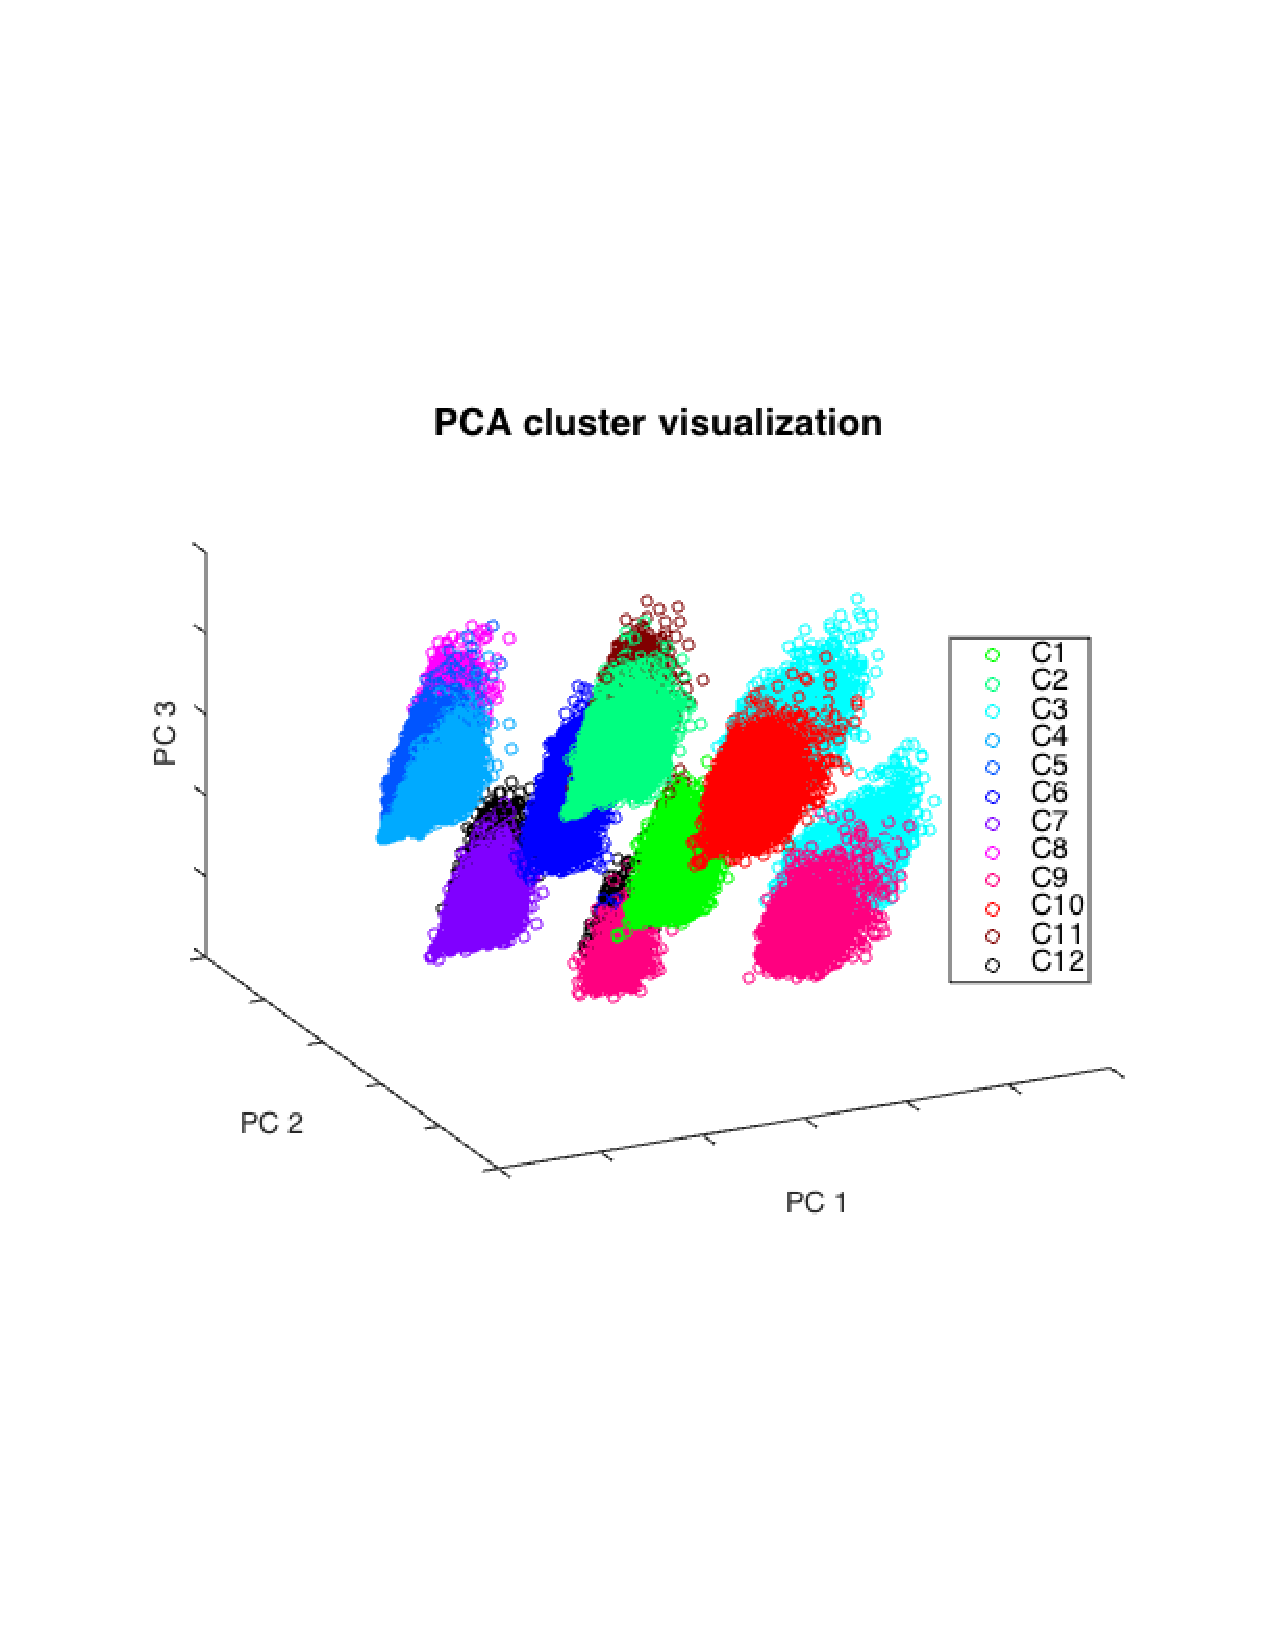
\includegraphics[trim=60pt 210pt 70pt 250pt, clip, width=0.8\textwidth]{viz-cluster.pdf}
    \label{fig:viz}
  \end{figure}
\end{itemize}

\medskip
\hrule\medskip
\Head{Game Outcome Prediction}

\begin{itemize}

  \item \textbf{Features} are team compositions for all teams in a game based on behavioral groupings generated from k-means and DP-means clustering

  \item \textbf{Labels} are win/loss for each game (if team 1 \emph{beats} team 2, label = 1)

  \item Classification algorithms (supervised learning)
  \begin{itemize}
    
    \item \textbf{Logistic regression} generalized linear model with Bernoulli distribution

    \item \textbf{Gaussian discriminant analysis} assuming data is Gaussian-distributed

    \item \textbf{Support vector machine} assuming data is separable by soft-margins

    \item \textbf{Cross validation} 10\% hold-out for all methods

  \end{itemize}

  \item \textbf{Best predictor} uses features based on k-means clustered team compositions for each game, trained on an SVM; 70.4\% accuracy (vs. 55.1\% baseline)

\end{itemize}

\medskip

\begin{table}[htbp!]
  \begin{minipage}{\textwidth}
    \centering
    \caption*{\textbf{Summary:} Outcome prediction algorithm results (10 trials average)}
    \begin{tabular}{lcccccc}
      \toprule
      & \multicolumn{2}{c}{k-means (\%)} & \multicolumn{2}{c}{DP-means (\%)} & \multicolumn{2}{c}{cpu time (s)} \\
      & train acc. & test acc. & train acc. & test acc. & k-means & DP-means \\ \midrule
      LR & 72.25 & 68.75 & 69.67 & 67.11 & 7.4 & 7.1 \\
      GDA & 74.79 & 70.14 & 70.88 & 68.39 & 7.7 & 7.1 \\
      SVM & 74.75 & 70.39 & 71.71 & 69.21 & 91.2 & 41.6 \\
      \bottomrule
    \end{tabular}
    \label{table:summary}
  \end{minipage} 
\end{table}

\medskip
\hrule\medskip
\Head{Conclusion and Extensions}

\begin{itemize}
  
  \item 

  \item 

  \item 

\end{itemize}

\medskip
\hrule\medskip
\Head{Acknowledgements}

We thank Professor Andrew Ng and the instructor team.

\end{textblock}

\end{document}
